
Der erste Teilversuch befasst sich mit sogenannten dichroitischen Spiegeln. Diese sind dünne Platten, welche in der Optomechatronik zur Aufspaltung farbigen Lichtes dienen. Erreicht wird dies durch Dünnfilminterferenz, welche bestimmte Wellenlängen reflektiert bzw. unbeeinflusst durch den Spiegel passieren lässt. Für den später betrachteten LCD-Beamer liefen diese Spiegel die verschiedenen Farben, und sind so integraler Bestandteil dessen Farbwiedergabe.

Es sollen zwei dieser Spiegel von den Teilnehmenden mithilfe eines Spektrometers untersucht werden, um deren Transmissionsspektren zu messen. Darauf folgend können die Reflektionsspektren der Spiegel bestimmt werden, um somit die Farbpositionen der reflektierten Lichtstrahlen im Farbdreieck zu bestimmen.

\subsubsection{Versuchsaufbau} Dieser besteht aus einer möglichst weißen, spektral verteilten Lichtquelle, hier einer LED mit Photphor. Das Licht der LED wird mithilfe eines Spiegels zu einem Strahl gebündelt, welcher auf die Messapertur eines Spektrometers gerichtet wird. Das Spektrometer ist von einem Computer aus bedienbar, und es können die gemessenen Spektren gespeichert werden. Zusätzlich steht den Teilnehmenden eine Halterung zur Verfügung, mit derer sich die dichroitischen Spiegel in den Lichtstrahl der LED, vor dem Spektrometer, in einem $45^\circ$-Winkel relativ zum Lichtstrahl befestigen lassen. Das reflektierte Licht wird auf eine weiße Abschirmung geworfen, um sichtbar gemacht zu werden.

\begin{figure}[h]
	\centering
	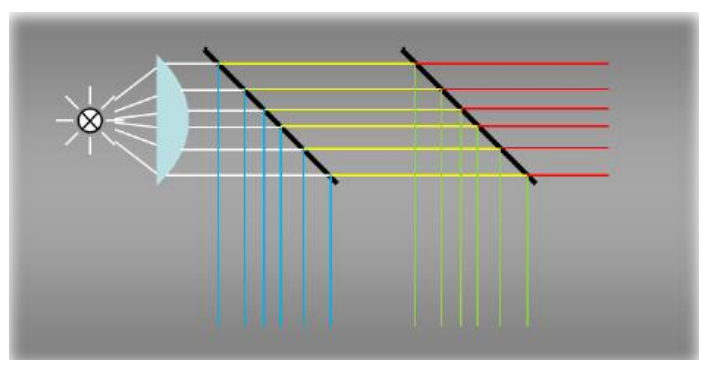
\includegraphics[scale=0.4]{Images/Aufbau.png}
	\caption{Schematischer Versuchsaufbau, [\cite[Abb. 3.2]{AML_SKRIPT}]}
\end{figure}

\subsubsection{Versuchsdurchführung}

Die Messung der Transmissionsspektren der Spiegel erfolgt in vier Schritten:
\begin{itemize}
\item Bestimmung einer Integrationszeit, bei welcher das Spektrometer zu ca. 75\% belichtet wird. Hierdurch wird eine Überbelichtung und somit Verfälschung der Messergebnisse verhindert. Im folgenden wird eine Integrationszeit von 90ms gewählt.
\item Durchführung einer Dunkelmessung des Hintergrundlichtes, um dieses aus den Messwerten entfernen zu können.
\item Durchführung einer Referenzmessung (100\%-Messung) der LED ohne eingebaute Spiegel. Mit dieser werden die späteren Messwerte automatisch normiert, um somit die relativen Anteile des transmittierten Lichtes berechnen zu können.
\item Messung der relativen Spektren von jeweils Spiegel 1 und Spiegel 1+2
\end{itemize}
In der folgenden Grafik sind die drei relevanten Kurven der relativen Spektren von Referenzmessung, von Spiegel 1 und von Spiegel 1+2 im sichtbaren Frequenzbereich dargestellt:

\begin{figure}[h]
	\centering
	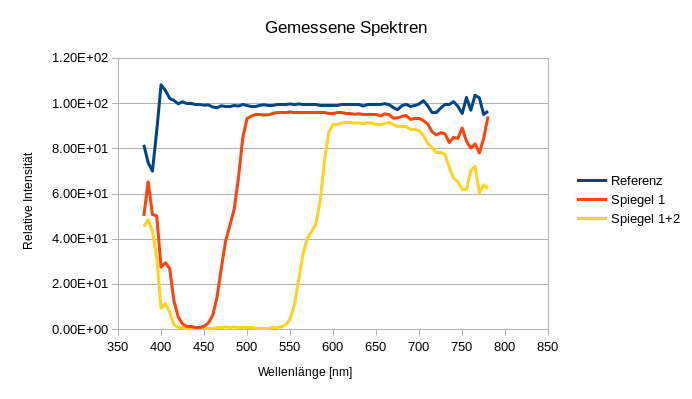
\includegraphics[scale=0.8]{Images/V1_Spektren.png}
	\caption{Relative Spektren der Spiegel im Vergleich}
	\label{V1_RES}
\end{figure}

\subsubsection{Auswertung}

\label{V1_AUSW}

Zuerst wird die Kurve der Referenzmessung betrachtet. Überwiegend liegt diese bei 100\%, wie es von der Referenzmessung zu erwarten ist. An der oberen und unteren Grenze des für den menschlich sichtbaren Wellenlängenbereiches kommt es jedoch zu Schwankungen. Diese lassen sich dadurch erklären, dass die verwendete LED in diesen Wellenlängen sehr schwach bis nicht leuchtet, und die Messwerte hierdurch stark vom Hintergrundrauschen beeinflusst werden. 

Das Spektrum des ersten Spiegels in Abb. \ref{V1_RES} lässt nun auf zweierlei schließen:
Die Transmission des Spiegels ist nicht vollständig, es wird anscheinen immer ein kleiner Teil des Lichtes reflektiert bzw. absorbiert. Erkennbar ist dies daran, dass die Kurve nie ganz 100\% erreicht. Zweitens ist deutlich der Bereich der Reflekion zwischen 400nm und 500nm zu erkennen, in welchem der Spiegel fast 100\% des Lichtes reflektiert. 

Schließlich wird das Spektrum beider Spiegel (1+2) betrachtet. Erstens ist zu erkennen dass es im Vergleich zu Spiegel 1 eine stärkere allgemeine Reflektion bzw. Absorption auch in nicht-reflektierten Wellenlängen gibt. Zweitens ist zu erkennen dass der zweite Spiegel einen Wellenlängenbereich von ca. 450nm bis 600nm reflektiert, da dort keines des vom Spiegel 1 durchgelassenen Lichtes mehr am Sensor an kommt.

Nun werden die jeweiligen relativen reflektierten Spektren der Spiegel ermittelt. Unter der Annahme dass das nicht tranmittierte Licht zu 100\% reflektiert wird, wird vom bekannten Referenzspektrum das Transmissionsspektrum des ersten Spiegels, bzw. vom Transmissionsspektrum des ersten Spiegels das Transmissionsspektrum des ersten und zweiten Spiegels abgezogen, und nach ersterem Spektrum normiert.

\begin{eqnarray}
	T_{\lambda, 1}(\lambda) = & D_{\lambda,0}(\lambda) - D_{\lambda,1}(\lambda) \\
	T_{\lambda, 2}(\lambda) = & D_{\lambda,1}(\lambda) - D_{\lambda,2}(\lambda) \\
	T_{\lambda, 3}(\lambda) = & D_{\lambda,3}(\lambda)
\end{eqnarray}
Es ergeben sich folgende Kurven:

\begin{figure}[h]
	\centering
	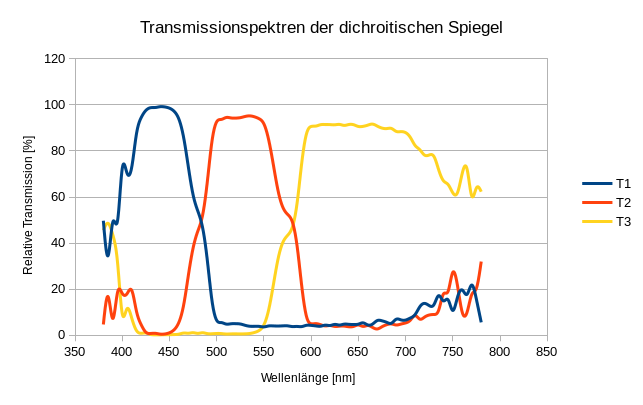
\includegraphics[scale=0.8]{Images/V2_Transmissionen.png}
	\caption{Berechnete relative Transmissionsspektren der aufgespalteten Strahlen}
	\label{V1_REFLECT}
\end{figure}

Die vorher vermuteten Reflektionsbereiche von 400nm bis 500nm bzw. 450nm bis 600nm sind hier gut erkennbar. Die starken Schwankungen des Reflektionsspektrums des zweiten Spiegels unter 450nm lassen sich durch niedrige absolute Werte erklären, welche somit stärker rauschen.
Das Verhalten der Spiegel kann somit als Bandpassfilter angenähert werden, welche für die obig genannten Wellenlängenbereiche das Licht reflektieren, ansonsten beinahe ungestört transmittieren.